% !TEX root =  main.tex

Communication-centered programming is playing a prominent role in the
production of nowadays software. Programming peers that need to
exchange information is an error-prone activity and the behaviour of
even small systems is subject to a combinatorial blow-up as the number
of peers increases.  Therefore well-structured principles and rigorous
foundations are needed to develop well-engineered, trustworthy
software.  One possibility is to exploit some sort of behavioural
types~\cite{DBLP:journals/csur/HuttelLVCCDMPRT16,dd09} to manage
abstract descriptions of peers and formally study their properties
such as communication safety, absence of deadlocks, progress or
session fidelity: given the types of the peers, the emerging behaviour
of their composition is analysed.  In the seminal
paper~\cite{DBLP:conf/popl/HondaYC08}, recently nominated the
\emph{most influential POPL paper (Award 2018)}, the authors push
forward an abstract notion of global type of interaction that
represents a sort of contract between the communicating peers. This is
paired with the notion of local type that gives an abstract
description of the behaviour of each peer, as taken in isolation.
Interestingly, local types can be obtained \quo{for free} by
projection from global types, while the properties of interest can be
studied and guaranteed just at the level of global types, without the
need of studying the composition of local types. The conformance of
peers implementation w.r.t. the global type can be studied instead at
the level of local types, allowing a more efficient form of type
checking. Roughly this means that properties are stated globally but
checked locally. Global types have been inspired by session
types~\cite{DBLP:conf/esop/HondaVK98} and by choreography languages in
service oriented computing
(WS-CDL\footnote{\url{http://www.w3.org/2002/ws/chor.}}), where
complex interactions are modelled from the point of view of the global
sequence of events that must take place in order to successfully
complete the computation.

In the literature, global/local types have been studied mostly in the
context of point-to-point channel-based interactions. This means that
the main action in a choreography is the sending of a message from one
peer to another on a specific channel (of a given type). In this paper
we explore a different setting, where interaction over tuple-spaces
replaces message passing, in the style of Linda-like
languages~\cite{DBLP:journals/toplas/Gelernter85}.  Instead of
primitives for sending and receiving messages, here there are
primitives for inserting a tuple on a tuple space, for reading
(without consuming) a tuple from a tuple space or for retrieving a
tuple from a tuple space. We call these interactions data-driven, as
decisions will be taken on the basis of the type of the tuples that
are manipulated.
%
We coined the term \emph{klaimographies} in honour of the process
language Klaim~\cite{DBLP:journals/tse/NicolaFP98,klaim}, a main
contribution of Rocco De Nicola in the fields of process algebras and
distributed programming.
%
Inspired by Klaim, klaimographies exploit the notion of distributed
tuple spaces to separate the access to data on the basis of the
interactions that are carried out.

% Localities can be communicated in tuples, allowing name mobility.
% 
\paragraph{A marketplace scenario}
We illustrate this with a motivating example that we will formalise
later (cf. \cref{ex:market} on page~\pageref{ex:market}).
%
We consider a scenario where sellers and buyers use a marketplace
provided by a broker.
%
Sellers can put on sale (several) items and buyers can inspect them.
%
When an item of interest is found, the client can start a negotiation
with the seller.
%
The intended behaviour of this choreography is informally represented
by the BPMN diagram\footnote{The diagram has been drawn with the tool
  BeePMN \url{https://www.beepmn.com}.} in \cref{fig:bpmn}.
%
\begin{figure}[t!]\centering
  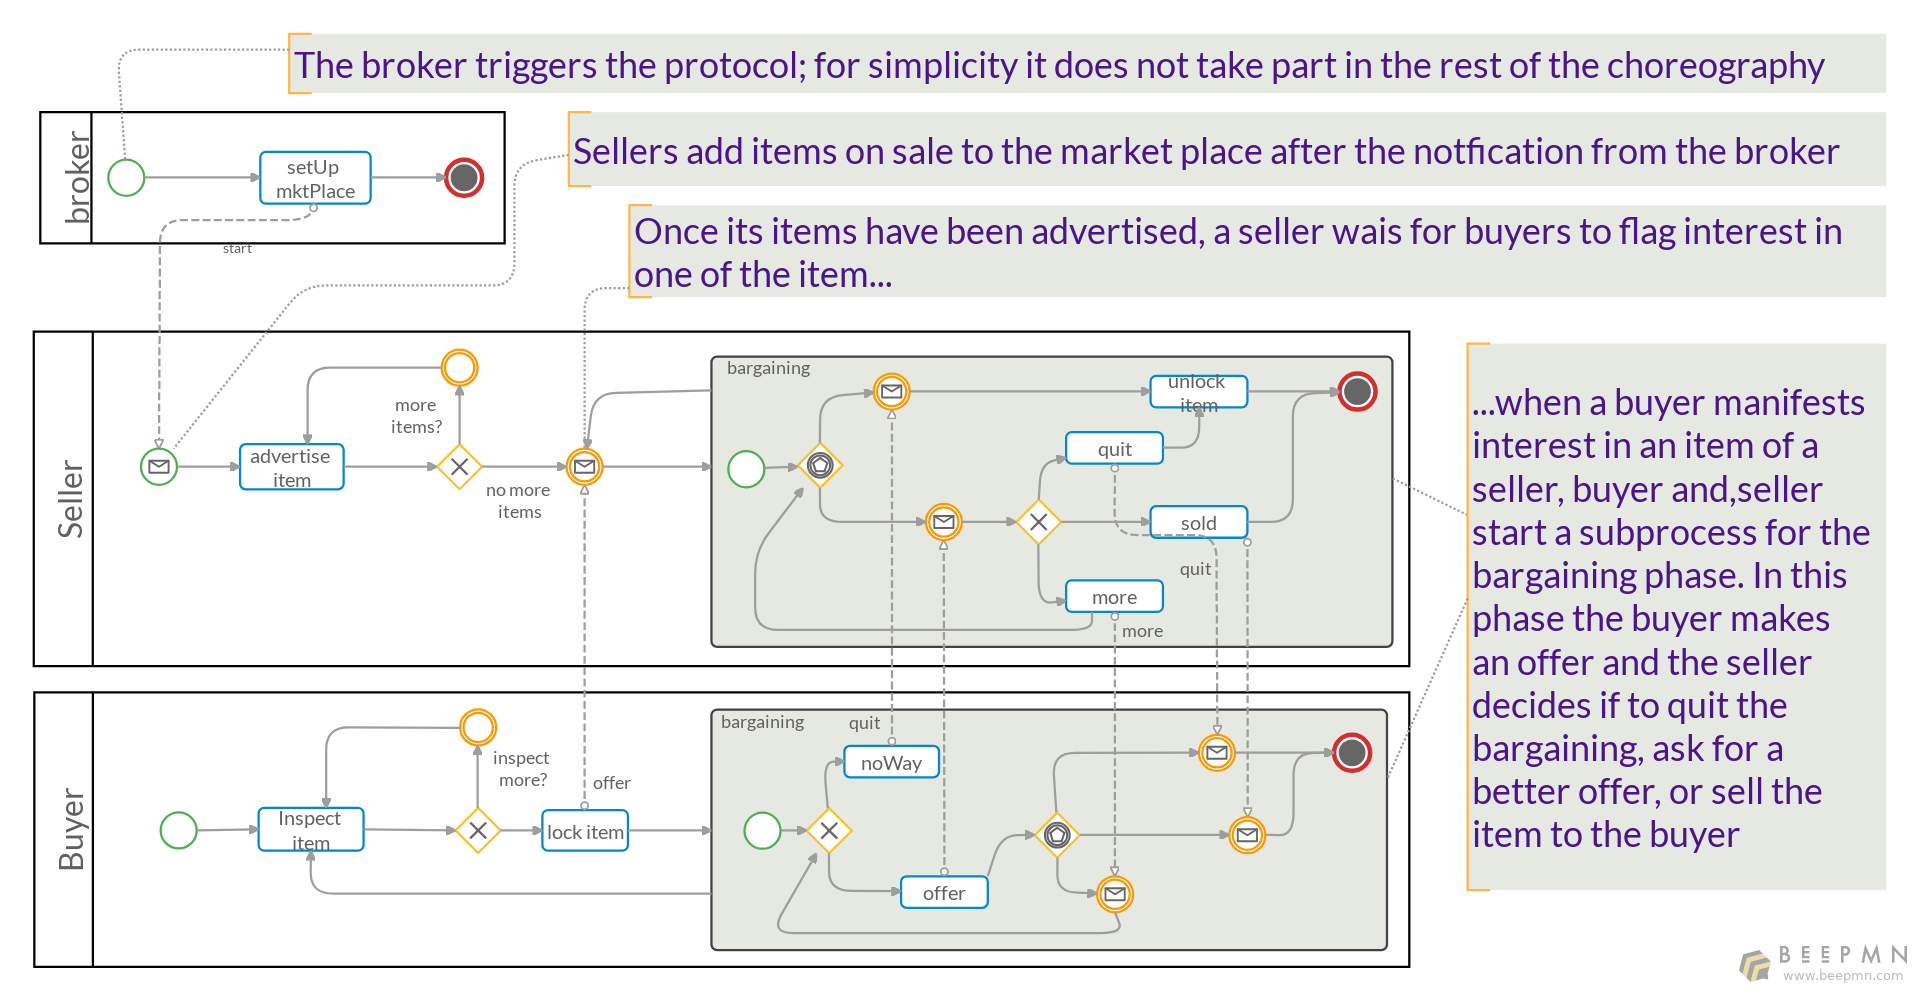
\includegraphics[scale=.18]{marketplace}
  \caption{A marketplace scenario\label{fig:bpmn}}
\end{figure}
%
The BPMN diagram though does not specify the protocol in a precise
way.
%
In our scenario there is a single broker but an arbitrary number of
sellers or buyers.
%
This is not reflected in the diagram because the BMPN pools `Seller'
and `Buyer' represent participants, not roles that maybe enacted by
many participants.
% 
Taking into account multiplicity of participants triggers interesting
issues.
% 
For instance, the bargaining subprocess should happen between two
specific instances of participants: the buyer interested in a
particular item and the seller that advertised such item.
% 
Moreover, the interactions among these specific instances must happen
without interference from other participants.

There are several distinguishing features of klaimographies w.r.t.
the literature on global types that tackle the issues described above.
%
First, klaimographies naturally support arbitrary number of
participants.
%
This is uncommon in standard behavioural types approaches where the
number of participants in interactions is usually fixed a priori, even
when the number of participants is a parameter of the type, as done
in~\cite{ydbh10} (see also \cref{sec:conc}).
%
Second, interactions of klaimographies are multiway because each tuple
can be read many times.
%
Typically, session types specify point-to-point interactions where
messages have exactly one producer and one consumer.
%
For instance, see~\cite{cdp12} and the discussions on multiway
interactions therein.
%
Third, all interactions involve a tuple space locality instead of a
channel name.
%
Fourth, klaimographies are data-driven in the sense that they
aim to check properties of data-flow.
%
An example of use of klaimographies is to control the access to pieces
of data in a tuple space.

The main contribution of this paper is to set up the formal setting of
klaimographies and to prepare the ground for several interesting
research directions: we fix the syntax of global and local types and
define the projection from global to local types, as typical of
choreographic frameworks.  Global types are equipped with a partial
order semantics of events and local types with an ordinary operational
semantics. Then, the conditions under which the behaviour of projected
local types is faithful to the semantics of global types are spelled
out.

Shifting the focus from control to data in choreographic framework has
several implications.
%
Firstly, the emphasis is no longer on properties related to
computational actors.
%
For instance, klaimographies admit computations where some processes
may not terminate and are left waiting for some data.
%
In standard choreographic frameworks those would be undesired behaviours
to rule out with suitable typing disciplines.
%
Nonetheless, we claim that in some application domains computations with
deadlocked processes have to be considered non-erroneous.
%
For instance, in reactive systems based on event-notification
frameworks some \quo{listener} components must be kept waiting for
events to occur.
%
Our work paves the way to the formal study of properties of data, like consumption, persistence and availability, in a choreographic setting.

Another main innovation of klaimographies is that they allow one to
easily represent protocols where a role can be enacted by an arbitrary
number of components.
%
We give an example of such protocol in \cref{sec:examples}.
%
Remarkably, those protocols can be specified in some existing
choreographic frameworks~\cite{ydbh10,chjny19}, but in a less abstract way
that requires the explicit quantification on components.

\paragraph{Structure of the paper.}
\todo{eM: revise} After some preliminaries in \cref{sec:tuples}, we
define klaimographies as global types in \cref{sec:gt} and give some
examples in \cref{sec:examples}.  In \cref{sec:globsem} we define the
semantics of global types and give the adequacy conditions for
projecting global types to local types.  In \cref{sec:locsem} we
define the syntax and operational semantics of local types and show
how to project global types over local types in \cref{sec:proj}.  The
semantic correspondence between global types and local types is
accounted for in \cref{sec:corr}.  Some concluding remarks together
with the discussion of related and future work are in \cref{sec:conc}.

%%% Local Variables:
%%% mode: latex
%%% TeX-master: "main"
%%% End:

